\documentclass{standalone}

\usepackage{tikz}
\usetikzlibrary{arrows,automata, positioning}
\usepackage{xcolor}
\definecolor{myblue}{RGB}{0,0,127} % navy blue


\begin{document}
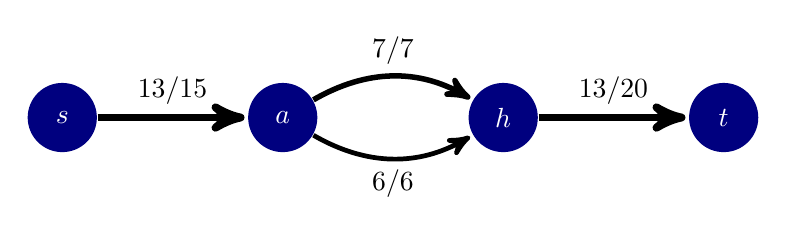
\begin{tikzpicture}[->,>=stealth',shorten >=1pt,auto,node distance=2.8cm, semithick]
  \tikzstyle{every state}=[fill=myblue,draw=none,text=white]

  \node[state]         (S)              {$s$};
  \node[state]         (A) [right of=S] {$a$};
  \node[state]         (H) [right of=A] {$h$};
  \node[state]         (T) [right of=H] {$t$};

  \path[line width=1.0mm] (S) edge [above] node {$13/15$} (A);
  \path[line width=0.7mm] (A) edge [bend left, above] node {$7/7$} (H);
  \path[line width=1.0mm] (H) edge              node {$13/20$} (T);
  \path[line width=0.6mm] (A) edge [bend right, below] node {$6/6$} (H);
\end{tikzpicture}
\end{document}
